\documentclass{beamer}
\mode<presentation>
\setbeamertemplate{navigation symbols}{}

% ----------------------------------------------------------------------
%footer
\setbeamertemplate{footline}
{
  \leavevmode
    \hfill
    \usebeamerfont{footer}
    ~~~~~~~~~~~~~~~~~~~~~~~~~~~~~~~~~~
    ~~~~~~~~~~~~~~~~~~~~~~~~~~~~~~~~~~
    \insertframenumber{} / \inserttotalframenumber
    ~~~~~
}

\usepackage[utf8]{inputenc}
\usepackage[T1]{fontenc}
\usepackage[french]{babel}

%figures
\usepackage{graphicx}
\graphicspath{{fig/}}
\DeclareGraphicsExtensions{.eps,.pdf,.jpg}
\usepackage{tikz}

%math
\usepackage{amssymb}
\usepackage{amsmath}
\usepackage{cancel}

% ----------------------------------------------------------------------
%macros

\newcommand{\Z}{{\ensuremath\mathbb{Z}}}
\newcommand{\N}{{\ensuremath\mathbb{N}}}
\newcommand{\R}{{\ensuremath\mathbb{R}}}

\renewcommand{\vec}[1]{\mathbf{#1}}
\newcommand{\ve}[1]{\ensuremath{\vec{e}_{#1}}}

% ----------------------------------------------------------------------
\title[]
 {4TC-IAT, Optimisation}

\author[T. Roussillon]
 {Tristan Roussillon}

\date{2020}

\institute{INSA Lyon, TC}

\begin{document}

% ----------------------------------------------------------------------
\begin{frame}
  \titlepage
\end{frame}

% ----------------------------------------------------------------------
\begin{frame}
  \frametitle{Introduction}

  \begin{block}{Les problèmes d'optimisation sont fréquents}
  \begin{itemize}
  \item à la question ``y a-t-il une solution ?'' (existence)
  \item suit ``quelle est la meilleure solution ?'' (optimisation)
  \item l'optimisation peut être sous-jacente : par ex., en apprentissage supervisé, on cherche
    une fonction de prédiction qui minimise une fonction de coût.
    %exemple du salaire d'une personne qui arrive
    %moyenne minimise les écarts quadratiques
    %mediane minimise les écarts absolus
    %mode, cad le plus probable. 
  \item certains problèmes sont difficiles et requièrent des méthodes inhabituelles pour découvrir
    des solutions, mêmes approchées : c'est une partie de ce qu'on appelle l'IA.
  \end{itemize}
  \end{block}
  
\end{frame}

% ----------------------------------------------------------------------
\begin{frame}
  \frametitle{Optimisation en télécommunications}

  \begin{itemize}
  \item Allocation de fréquences / channel assignment
    %Global System for Mobile Communications (GSM) (historiquement « Groupe spécial mobile »1)
    %est une norme numérique de seconde génération pour la téléphonie mobile
  \item Allocation de canaux / time slot assignment
    %% Le time division multiple access (TDMA) ou accès multiple à répartition dans le temps en français, est une technique de contrôle d'accès au support permettant de transmettre plusieurs flux de trafic sur un seul canal ou une seule bande de fréquence. Il utilise une division temporelle de la bande passante, dont le principe est de répartir le temps disponible entre les différents utilisateurs. Par ce moyen, une fréquence (porteuse) ou une longueur d'onde peut être allouée, à tour de rôle (quasi simultanément), à plusieurs abonnés. 
  \item Routage et allocation de longueurs d'onde / routing and wavelength assignment
    %multiplexage en longueur d'onde, souvent appelé WDM (Wavelength Division Multiplexing en anglais)
  \item Routage IP
  \item Optimisation dans les réseaux radio maillés :
    \begin{itemize}
    \item placement min. de points d'accès / min. gateway placement
    \item placement équitable de points d'accès / fair gateway placement
    \item routage équitable / fair joint routing and scheduling
    \item routage en temps minimum / minimum time routing
    \end{itemize}
    %p. 36/37 thèse Optimisation de la capacité des réseaux maillés, C. Molle  
  \end{itemize}
  
\end{frame}

% ----------------------------------------------------------------------
\section{\'Enoncé du problème}
% ----------------------------------------------------------------------

\begin{frame}
  \frametitle{Problème d'optimisation}

  \[
  \text{(P)} \left\{
  \begin{array}{c}
    \text{min} \ f(x) \ \text{tel que :} \\
    g_i(x) \leq 0, \ i \in I = \{1, \dots, m\} \\
    x \in S \subseteq \R^n
  \end{array}
  \right.
  \]

  \only<1>{
    \begin{block}{Vocabulaire}
    \begin{itemize}
    \item fonction objectif : $f : \R^n \rightarrow \R$
    \item inconnues : composantes du vecteur $x^T := (x_1, \dots, x_n) \in \R^n$
    \item contraintes : $(g_i)_{i \in I}$ et $x \in S$
    \item une solution (candidate) : $x$ satisfaisant les contraintes
    \item solution optimale/optimum global : une solution minimisant $f$
    \end{itemize}
    %distinction des contraintes en deux:
    %- generalisation a plusieurs classes de pb
    %- traites differement dans les algos
    \end{block}
  }
  \only<2>{
    \begin{block}{Remarques}
    \begin{itemize}
    \item nombre d'inconnues $n \geq 1$ 
    \item max $f'$ $\Leftrightarrow$ min $-f'$
    \item sans contrainte ($I = \emptyset$) ou avec ($I \neq \emptyset$)
    \item contraintes d'égalité $g'(x) = 0$ $\Leftrightarrow$ $g'(x) \leq 0$ et $-g'(x) \leq 0$
    \item généralement pas d'inégalités strictes
    \end{itemize}
    \end{block}
    %existence de solution (th. de Weierstrass)
    %si f est une fonction reelle continue sur K \subset R^n ferme et borne, alors il existe
    %une solution optimale x \in K qui min f(x)
    %existence aussi si f est une fonction reelle continue et possède la propriété de croissance à l'infini:
    %f(x) -> +inf qs x -> +inf
    %inégalités strictes => ensemble de solutions non ferme et borne, donc possiblement pas de solutions. 
  }
  \only<3->{
    \begin{block}{Résoudre (P) peut être difficile...}
    \begin{itemize}
    \item $n$ peut être grand
    \item l'ensemble des solutions peut être vide, très grand ou infini
    \item $f$ et les $g_i$ peuvent être quelconques %ni differentiable, ni convexe, ni lineaire
    \item $f$ peut être (quasiment) plat autour du min
      %si plat, plusieurs solutions optimales, si quasiment, instabilités numériques 
    \item $f$ peut ne pas être analytiquement connu 
    \end{itemize}
    \end{block}
  }
\end{frame}

\begin{frame}
  \frametitle{Optimum local vs optimum global}

  \begin{block}{Définition}
    La solution $x^0$ est un optimum local du problème (P) s'il existe un voisinage
    $V(x^0)$ autour de $x^0$ tel que $x^0$ soit optimum global du problème
  \[
  \left\{
  \begin{array}{c}
    \text{min} \ f(x) \ \text{tel que :} \\
    g_i(x) \leq 0, \ i = 1, \dots, m \\
    x \in S \alert{\cap V(x^0)}
  \end{array}
  \right.
  \]
  \end{block}

  \begin{exampleblock}{Exemple dans $\R$}
    \centering
    \includegraphics[width=0.7\textwidth]{opt-loc}
  \end{exampleblock}
  
\end{frame}

% ----------------------------------------------------------------------
\section{Convexité et différentiabilité}
% ----------------------------------------------------------------------
%permet de dire si on peut chercher un min ou un max
%permet de dire si tout optimum local est un optimum global ou non

% ----------------------------------------------------------------------
\begin{frame}<beamer>
  \frametitle{Sommaire}
  \tableofcontents[currentsection]
\end{frame}


% ----------------------------------------------------------------------
\begin{frame}
  \frametitle{Convexité d'un ensemble}

  \begin{block}{Définition}
    $S \subset \R^n$ est convexe ssi  
    pour tout $x,y \in S$ et $\lambda \in [0,1]$,
    $\lambda x - (1 - \lambda) y \in S$. 
  \end{block}

  \begin{exampleblock}{Exemple pour $S \subset \R^2$}
    \centering
    \includegraphics[width=0.25\textwidth,page=1]{ens-conv} \hspace{0.05\textwidth}
    \includegraphics[width=0.25\textwidth,page=2]{ens-conv}
  \end{exampleblock}
  
\end{frame}

% ----------------------------------------------------------------------
\begin{frame}
  \frametitle{Convexité d'une fonction}

  \begin{block}{Définition}
     Soit $S \subset \R^n$ convexe.
     Une fonction $f : S \rightarrow \R$ est convexe ssi  
    pour tout $x,y \in S$ et $\lambda \in [0,1]$,
    $f(\lambda x - (1 - \lambda) y) \leq \lambda f(x) + (1 - \lambda) f(y)$. 
  \end{block}

  \begin{exampleblock}{Exemple pour $f:\R \rightarrow \R$}
    \centering
    \includegraphics[width=0.45\textwidth,page=1]{fonc-conv} \hspace{0.05\textwidth}
    \includegraphics[width=0.45\textwidth,page=2]{fonc-conv}
  \end{exampleblock}
  
\end{frame}

% ----------------------------------------------------------------------
\begin{frame}
  \frametitle{Différentiabilité pour $f: \R \rightarrow \R$}

  \begin{block}{Dérivée première}
    $f'(x) := \frac{\partial f}{\partial x} = \lim_{h \rightarrow 0} \frac{f(x+h) - f(x)}{h}$.\\
    Géométriquement, c'est la pente de la tangente au graphe de $f$ 
  \end{block}

  {
    \begin{center}
      \includegraphics<+>[width=0.5\textwidth,page=1]{derivee}    
      \includegraphics<+>[width=0.5\textwidth,page=2]{derivee}
    \end{center}
  }
  
  \begin{block}{Dérivée seconde = dérivée de la dérivée première}
    $f''(x) := \frac{\partial f'}{\partial x} = \frac{\partial ^{2}f}{\partial x^{2}}$.
  \end{block}
  
\end{frame}

% ----------------------------------------------------------------------
\begin{frame}
  \frametitle{Différentiabilité pour $f: \R^n \rightarrow \R$}
  
  \begin{block}{Gradient (vecteur), extension de la dérivée première}
    ${\nabla f}^T := (\frac{\partial f}{\partial x_1}, \frac{\partial f}{\partial x_2}, \dots, \frac{\partial f}{\partial x_n})$ \\
    Géométriquement, il est perpendiculaire à la courbe de niveau projetée. 
  \end{block}

  \only<1>{
    \begin{center}
      \includegraphics<+>[width=0.9\textwidth]{gradient}    
    \end{center}
  }
  \only<2>{
    \begin{block}{Hessien (matrice), extension de la dérivée seconde}
      $\nabla^2 f :=
      \begin{bmatrix}{\frac {\partial ^{2}f}{\partial x_{1}^{2}}}&{\frac {\partial ^{2}f}{\partial x_{1}\partial x_{2}}}&\cdots &{\frac {\partial ^{2}f}{\partial x_{1}\partial x_{n}}}\\{\frac {\partial ^{2}f}{\partial x_{2}\partial x_{1}}}&{\frac {\partial ^{2}f}{\partial x_{2}^{2}}}&\cdots &{\frac {\partial ^{2}f}{\partial x_{2}\partial x_{n}}}\\\vdots &\vdots &\ddots &\vdots \\{\frac {\partial ^{2}f}{\partial x_{n}\partial x_{1}}}&{\frac {\partial ^{2}f}{\partial x_{n}\partial x_{2}}}&\cdots &{\frac {\partial ^{2}f}{\partial x_{n}^{2}}}\end{bmatrix}$
    \end{block}
  }
\end{frame}


% ----------------------------------------------------------------------
\begin{frame}
  \frametitle{Différentiabilité et convexité}

  \begin{block}{Théorème}
    Si $f$ est continûment différentiable (deux fois), les conditions 1, 2 (et 3) sont équivalentes:
    \begin{enumerate}
    \item $f$ est convexe,
    \item $\forall x, y, \ f(y) > f(x) + {\nabla f} ^T(x) \cdot (y - x)$,
    \item $\forall x$, le hessien $\nabla^2f(x)$ est une matrice \emph{semi-définie positive},
      c-à-d. ses valeurs propres sont \emph{positives ou nulles}.
    \end{enumerate}
  \end{block}

  \begin{block}{Note:}
    Les valeurs propres d'une matrice carrée sont les composantes du vecteur
    $\lambda^T := (\lambda_1, \lambda_2,\dots, \lambda_n)$, solutions de
    l'équation $\det{(\nabla^2f(x) - \lambda I)}$.  
  \end{block}

\end{frame}

% ----------------------------------------------------------------------
\begin{frame}
  \frametitle{Conditions d'optimalité générales}

  \begin{block}{Conditions d'optimalité locale}
    Soit $f$ continue et deux fois continûment différentiable en tout $x \in \R^n$.
    $x^\star$ est un optimum local ssi
    \begin{itemize}
    \item ${\nabla f}^T(x^\star) = 0$ (stationnarité) et
    \item $\nabla^2f(x^\star)$ est une matrice \emph{définie positive},
      c-à-d. ses valeurs propres sont \emph{strictement positives}.
      %le strictement permet d'éviter les points d'inflexion ou
      %on a un point stationnaire et ou le hessien est seulement semi-definie positive
    \end{itemize}
  \end{block}

  \only<1>{
  \begin{block}{Théorème d'optimalité globale (avec différentiabilité)}
    Soit $f$ convexe et continûment différentiable en tout $x \in \R^n$.
    $x^\star$ est un optimum global ssi ${\nabla f}^T(x^\star) = 0$.
  \end{block}
  }
  \only<2>{
  \begin{block}{Théorème d'optimalité globale (sans différentiabilité)}
    Soit $f$ convexe et définie sur $S \subset \R^n$ convexe.
    Tout optimum local est un optimum global.  
  \end{block}
  }
  
\end{frame}

% ----------------------------------------------------------------------
\begin{frame}
  \frametitle{Exemple numérique pour $f:\R \rightarrow \R$}

    \only<1>{
      $f(x) = x^2 - 6x + 4$\\
      $f'(x) = 2x - 6$\\
      $f''(x) = 2$ \\ 
      ~\\
      $\forall x, \ f''(x) > 0 \Rightarrow f$ convexe $\Rightarrow$ $\exists$ un minimum global $x^\star$ tel que:
      $f'(x^\star) = 0 \Leftrightarrow x^\star = 3$.
    }
    \only<2>{
      $f(x) = 2x^3 - x^2 + 2x + 5$\\
      $f'(x) = 6x^2 - 2x + 2$\\
      $f''(x) = 12x - 2$ \\ 
      ~\\
      On ne peut rien dire de la convexité pour tout $x$.\\
      Mais on peut procéder par intervalle. 
    }
  
\end{frame}

% ----------------------------------------------------------------------
\begin{frame}
  \frametitle{Exemple numérique pour $f:\R^2 \rightarrow \R$}

  \begin{itemize}
  \item $f(x_1,x_2) = x_1^2 + x_2^2 - 4x_1 + 8x_2 - 5$
  \item $\frac{\partial f}{\partial x_1} = 2x_1 - 4, \frac{\partial f}{\partial x_2} = 2x_2 + 8$
  \item $\frac{\partial^2 f}{\partial x_1^2} = 2, \frac{\partial^2 f}{\partial x_1x_2} = 0, \frac{\partial^2 f}{\partial x_2x_1} = 0, \frac{\partial^2 f}{\partial x_2^2} = 2$
  \end{itemize}

  
  $\forall (x_1,x_2), \ \nabla^2f(x_1,x_2) =
  \left(\begin{array}{cc}
    2 & 0 \\
    0 & 2 \\
  \end{array}
  \right)
  $ $\Rightarrow$ $f$ est convexe $\Rightarrow$ \\
  $\exists$ un minimum global $x^\star$ tel que ${\nabla f}^T(x^\star) = 0$, c-à-d.
  \[
  \left\{
  \begin{array}{ll}
    2x^\star_1 - 4 & = 0\\
    2x^\star_2 + 8 & = 0
  \end{array}
  \right.
  \Leftrightarrow x^\star = (2,-4).
  \]
  
\end{frame}


% ----------------------------------------------------------------------
\section{Optimisation sans contrainte}
% ----------------------------------------------------------------------

% ----------------------------------------------------------------------
\begin{frame}<beamer>
  \frametitle{Sommaire}
  \tableofcontents[currentsection]
\end{frame}

% ----------------------------------------------------------------------
\begin{frame}
  \frametitle{Enoncé du problème}

  \[
  (\text{P}^\circ) \quad
    \text{min} \ f(x), \ x \in \R^n
  \]

  \begin{itemize}
  \item problème fréquent,
  \item même avec contraintes, on peut parfois se ramener à $\text{P}^\circ$,
  \item existence d'une solution optimale si $f$ est continue et :
    \begin{itemize}
    \item soit est définie dans $S \subset \R^n$, fermé et borné,
    \item soit $f(x) \rightarrow \infty$ quand $\|x\| \rightarrow \infty$, 
    \end{itemize}
  \item mais non unicité et nombreux optima locaux pour $f$ quelconque.
  \end{itemize}
  
\end{frame}

% ----------------------------------------------------------------------
\begin{frame}
  \frametitle{Schéma général de la descente de gradient}

  \begin{itemize}
  \item Soit $f : \R^n \rightarrow \R$ (+ hypothèses)
  \item On part d'une solution initiale $x^{(0)}$
  \item A chaque étape, on obtient une nouvelle solution
    \[ x^{(k+1)} := x^{(k)} - \textcolor{blue}{\lambda^{(k)}} \alert{{\nabla f}(x^{(k)})}, \ \lambda^{(k)} > 0. \]
    (c-à-d. qu'on se déplace dans la direction opposée du \alert{gradient},
    d'un pas d'une certaine \textcolor{blue}{longueur})
  \item On s'arrête quand le gradient s'annule (ou presque)
  \end{itemize}

  ~

  Questions : 
  terminaison ?
  solution initiale ?
  longueur du pas ?
\end{frame}

% ----------------------------------------------------------------------
\begin{frame}
  \frametitle{La terminaison dépend de $f$ et de la solution initiale}

  \begin{itemize}
    \item $f(x) = 2x\exp{(-x^2)}$
  \end{itemize}
  
  \begin{center}
      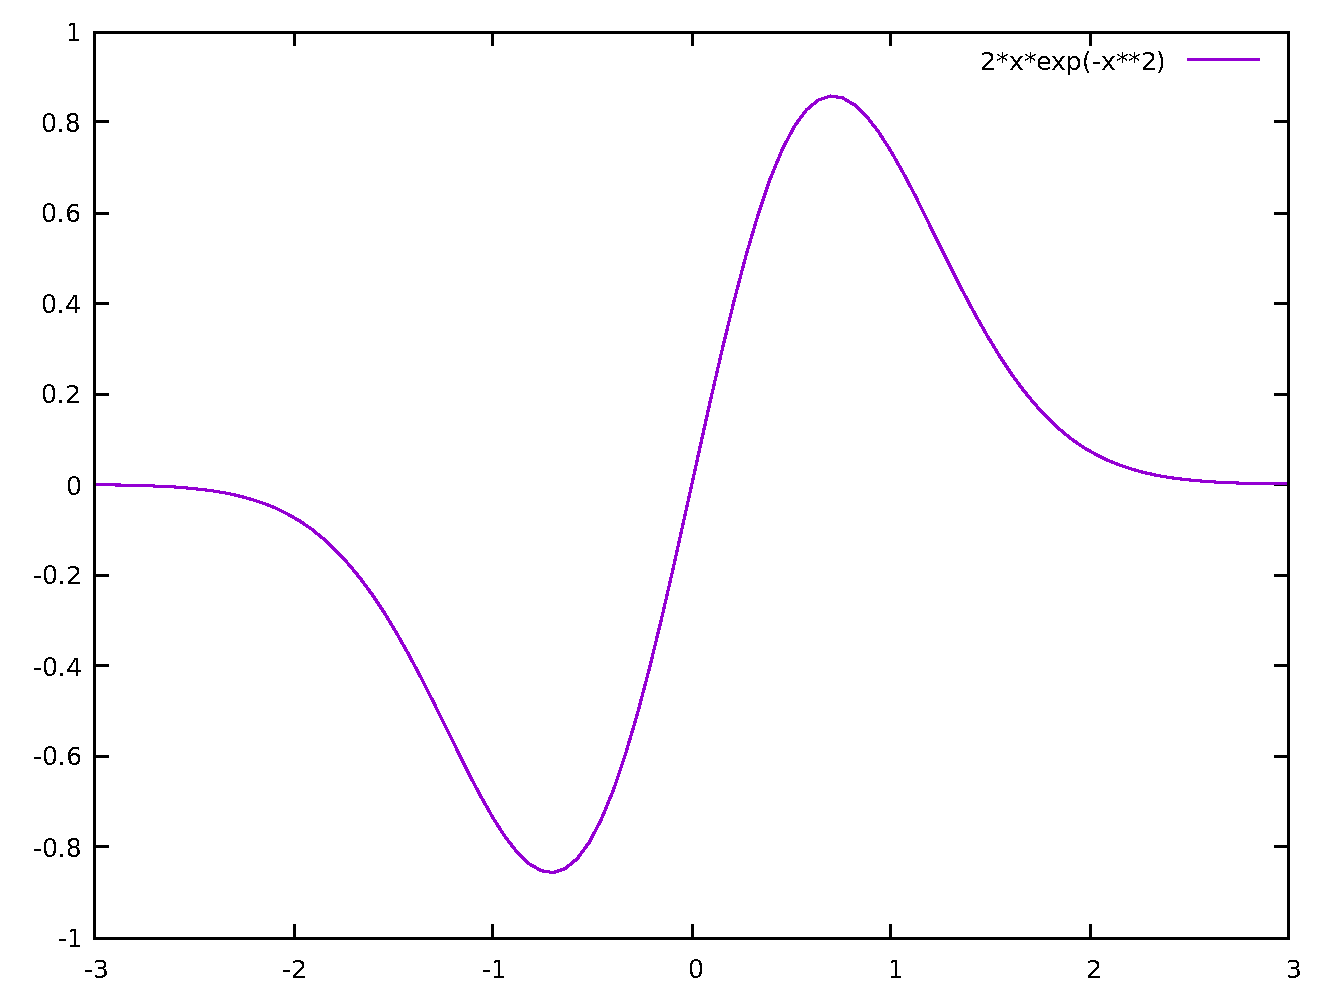
\includegraphics[width=0.6\textwidth]{desc-grad-non-conv}    
  \end{center}
  
  \begin{itemize}
  \item En partant de $x^{(0)} = 0$, on peut atteindre $-\frac{\sqrt{2}}{2}$, le minimum.
  \item En partant de $x^{(0)} = 1$, on a $x^{(k)} \rightarrow \infty$ quand $k \rightarrow \infty$. 
  \end{itemize}
  
\end{frame}


% ----------------------------------------------------------------------
\begin{frame}
  \frametitle{Longueur du pas}

  \begin{block}{De nombreuses méthodes pour déterminer $\lambda^{(k)}$}
  \begin{itemize}
  \item fixé par l'utilisateur (mais normalisé par la norme du gradient)
  \item $1 / k \|{\nabla f}(x^{(k)})\|$ (le pas diminue au fur et à mesure des itérations)
  \item \emph{Newton}: $\Big( {\nabla^2 f}(x^{(k)}) \Big)^{-1}$
    \begin{itemize}
    \item $x^{(k+1)}$ est l'optimal d'une approximation quadratique en $x^{(k)}$
    \item nécessite le hessien (et le gradient)
    \end{itemize}
  \item \emph{Steepest descent}: tel que $f(x^{(k)} - \lambda^{(k)} {\nabla f}(x^{(k)}))
    = \min_{\lambda \geq 0} f(x^{(k)} - \lambda {\nabla f}(x^{(k)}))$
  \end{itemize}
  \end{block}
\end{frame}

% ----------------------------------------------------------------------
\begin{frame}
  \frametitle{Méthode de Newton: convergence en un pas}

  \begin{itemize}
  \item $f(x_1,x_2) = a_1x_1^2 + b_1x_1 + c_1 + a_2x_2^2 + b_2 + c_2$
  \item %$\frac{\partial f}{\partial x_1} = 2a_1x_1 + b_1, \frac{\partial f}{\partial x_2} = 2a_2x_2 + b_2$
    %, donc
    $\forall (x_1,x_2), \ {\nabla f}(x_1,x_2)^T = (2a_1x_1 + b_1,2a_2x_2 + b_2)$
  \item %$\frac{\partial^2 f}{\partial x_1^2} = 2a_1, \frac{\partial^2 f}{\partial x_1x_2} = 0,
    %\frac{\partial^2 f}{\partial x_2x_1} = 0, \frac{\partial^2 f}{\partial x_2^2} = 2a_2$, donc
  $ \forall (x_1,x_2), \ \nabla^2f(x_1,x_2) =
  \left(\begin{array}{cc}
    2a_1 & 0 \\
    0 & 2a_2 \\
  \end{array}
  \right)
  $
  %
  \end{itemize}

  \begin{itemize}
  \item $\left( \begin{array}{c} x_1^{(1)} \\ x_2^{(1)} \end{array} \right ) =
    \left( \begin{array}{c} x_1^{(0)} \\ x_2^{(0)} \end{array} \right ) -
  \left(\begin{array}{cc} \frac{1}{2a_1} & 0 \\ 0 & \frac{1}{2a_2} \\ \end{array} \right) \cdot
  \left( \begin{array}{c} 2a_1x_1^{(0)} + b_1 \\ 2a_2x_2^{(0)} + b_2 \end{array} \right ) =
  \left( \begin{array}{c} -\frac{b_1}{2a_1} \\ -\frac{b_2}{2a_2} \end{array} \right ) $, or
  ${\nabla f}(-\frac{b_1}{2a_1}, -\frac{b_2}{2a_2})$ est nul : on a le minimum
  \item \alert{convergence en une itération car $f$ est quadratique et convexe}
  \end{itemize}
  
\end{frame}

% ----------------------------------------------------------------------
\begin{frame}
  \frametitle{Méthode de Newton: non convergence}

  \begin{itemize}
  \item $f(x) = \left \{
    \begin{array}{ll}
      -4x^3 + 3x^4 & \text{si} \ x\geq 0 \\
      4x^3 + 3x^4 & \text{si} \ x < 0 \\
    \end{array} \right.$
  \end{itemize}
  
  \begin{center}
      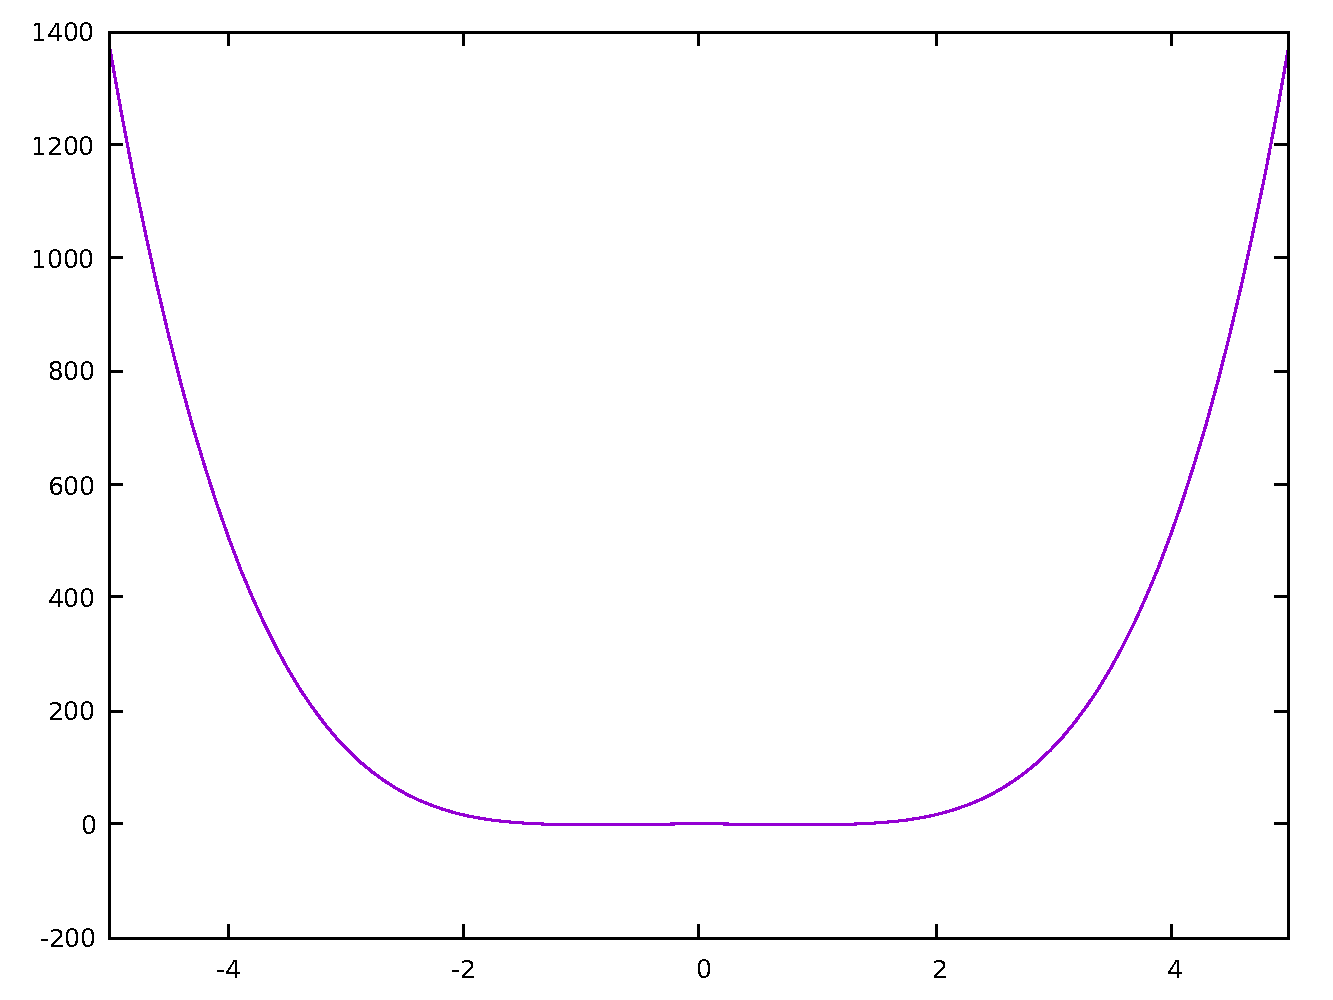
\includegraphics[width=0.6\textwidth]{newton-non-conv}    
  \end{center}
  
  \begin{itemize}
  \item En partant de $x^{(0)} = 0.4$, on converge vers 0, le minimum.
  \item En partant de $x^{(0)} = 0.6$, on a $x^{(1)}$ = -0.6, $x^{(2)}$ = 0.6\dots 
  \end{itemize}
  
\end{frame}

% ----------------------------------------------------------------------
\begin{frame}
  \frametitle{\emph{Steepest Descent}: convergence lente}

  \begin{itemize}
  \item $f(x_1,x_2) = 2x_1x_2 + 2x_2 - x_1^2 - 2x_2^2$
  \item$(x_1^{(0)}, x_2^{(0)}) = (0, 0.5)$ 
  \end{itemize}

  \begin{center}
      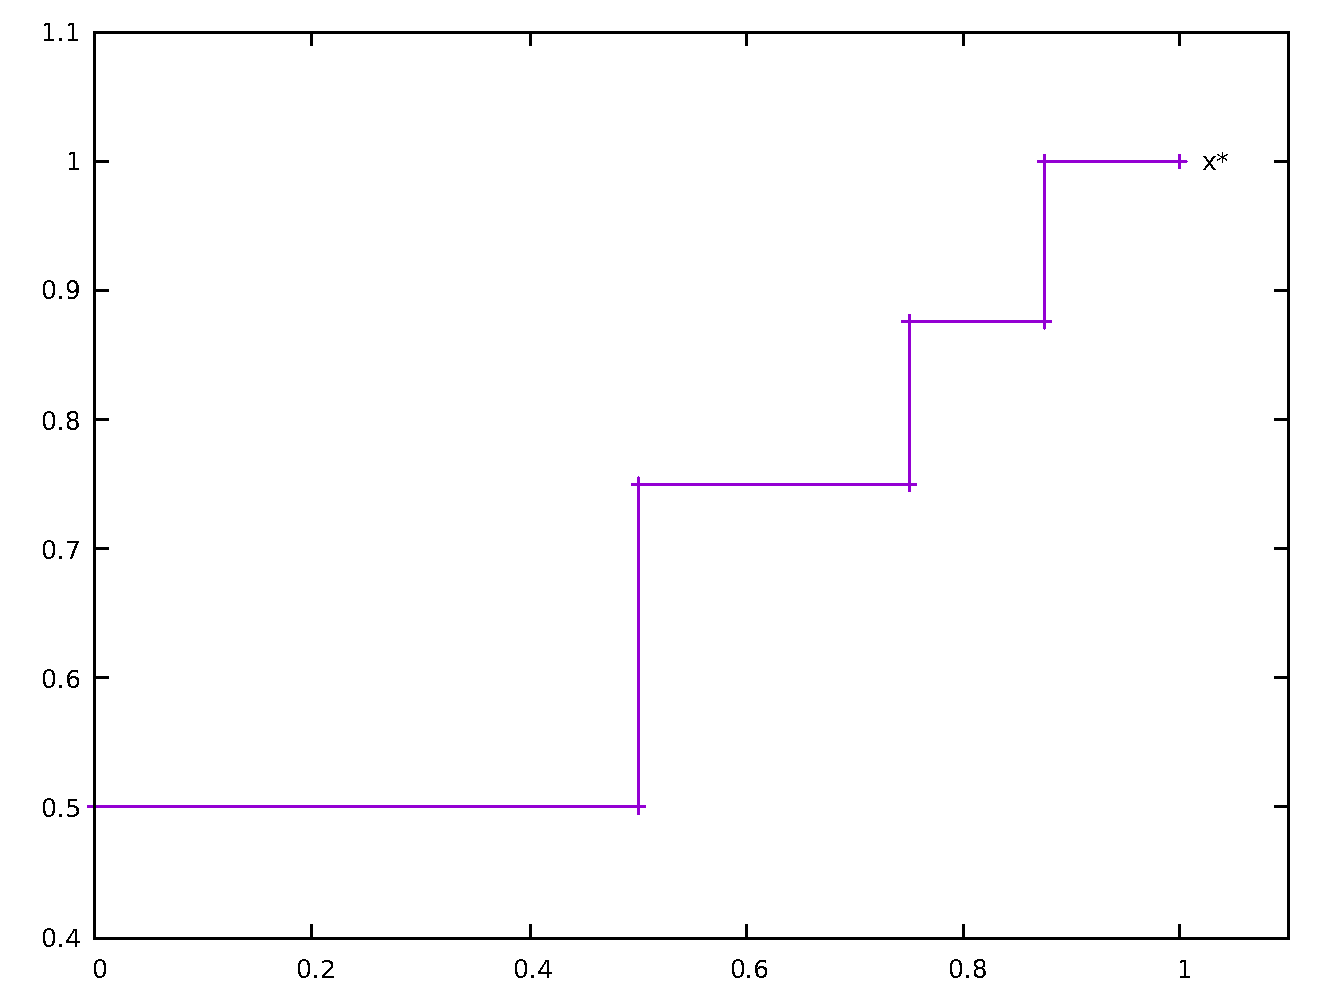
\includegraphics[width=0.6\textwidth]{steepest-desc}    
  \end{center}
  
  \begin{itemize}
  \item Deux directions successives sont toujours orthogonales
  \item Ce qui est lent pour des fonctions à \emph{vallée étroite}. 
  \end{itemize}
    
  
\end{frame}

% ----------------------------------------------------------------------
\begin{frame}
  \frametitle{Autres méthodes}

  \begin{itemize}
  \item Newton modifié et quasi-Newton
  \item méthode du gradient conjugué, méthode de Fletcher et Reeves
  \item méthode de Davidon-Fletcher-Powell (DFP)
  \item méthode de Broyden-Fletcher-Goldfarb-Shanno (BFGS)
  \item algorithme de Powell (sans dérivée !)
  \end{itemize}
  
\end{frame}

% ----------------------------------------------------------------------
\begin{frame}
  \frametitle{Cas d'une somme de fonctions (cf. TD)}

  \[
  (\text{P}^\circ) \quad
    \text{min} \ f(x) := \sum_{i = \{1,\dots,l\}} q_i(x), \ x \in \R^n
  \]

  \[ x^{(k+1)} := x^{(k)} - \lambda^{(k)} {\nabla f}(x^{(k)}), \ \lambda^{(k)} > 0. \]
  
  \begin{itemize}
  \item méthode du gradient stochastique : on évalue le gradient
    \begin{itemize}
    \item sur 1 fonction $q_i(x), \ i \in \{1,\dots,l\}$ au hasard
    \item ou sur plusieurs (\emph{mini-batch}), mais pas sur tout $f$
    \end{itemize}
  \item variantes :
    \begin{itemize}
    \item méthode du moment 
    \item RMSprop
    \item Adam
    \end{itemize}
  \end{itemize}
  
\end{frame}

%%40 min

% ----------------------------------------------------------------------
\section{Optimisation avec contraintes}
% ----------------------------------------------------------------------

% ----------------------------------------------------------------------
\begin{frame}<beamer>
  \frametitle{Sommaire}
  \tableofcontents[currentsection]
\end{frame}

% ----------------------------------------------------------------------
\begin{frame}
  \frametitle{\'Enoncé du problème}

  \[
  (\text{P}^\bullet) \left\{
  \begin{array}{c}
    \text{min} \ f(x) \ \text{tel que :} \\
    g_i(x) \leq 0, \ i \in I = \{1, \dots, m\} \\
    x \in \R^n
  \end{array}
  \right.
  \]

  \begin{block}{Hypothèses}
    \begin{itemize}
    \item (H1) $f$ et $(g_i)_{i \in I}$ continues, différentiables
    \item (H2) $X = \{ x \in \R^n \ | \ g_i(x) \leq 0, i \in I = \{1, \dots, m\} \}$,
      l'ensemble des solutions de $(\text{P}^\bullet)$ est non vide, mais peut avoir un
      intérieur vide, c-à-d. il n'existe pas de $x_0$ vérfiant $g_i(x_0) < 0, \ \forall i \in I$
    \item (QC) \alert{hypothèse de qualification des contraintes}
    \end{itemize}
  \end{block}
  
\end{frame}

% ----------------------------------------------------------------------
\begin{frame}
  \frametitle{Saturation et cône tangent en un point $x_0 \in X$}

  \begin{itemize}
    \item Une contrainte $g_i$ est \emph{saturée} ssi $g_i(x_0) = 0$
    \item L'ensemble des contraintes saturées en $x_0$ est
      $\{g_i\}_{i \in I_0}, \ I_0 := \{i \ | \ g_i(x_0) = 0 \}$
    \item Le cône tangent en $x_0$ est donné par le gradient des contraintes saturées en $x_0$ :
      $G_0 := \{ y \in \R^n \ | \ {\nabla g_i}^T \cdot y \leq 0, \ \forall i \in I_0 \}$ 
  \end{itemize}

  \begin{center}
      \includegraphics[width=0.45\textwidth,page=1]{cone-tangent} \hspace{0.01\textwidth}   
      \includegraphics[width=0.45\textwidth,page=2]{cone-tangent}    
  \end{center}
  
\end{frame}

% ----------------------------------------------------------------------
\begin{frame}
  \frametitle{Hypothèse de qualification des contraintes (QC)}

$X$ satisfait en $x^0 \in X$ l'hypothèse (QC) ssi 
  on peut se déplacer de $x_0$ vers tout point de $G_0$ suffisamment proche en restant dans $X$.

  \only<1>{
  \begin{exampleblock}{Cas où (QC) est vérifiée en $x_0$ : }
  \begin{center}
      \includegraphics[width=0.5\textwidth,page=1]{cone-tangent}    
  \end{center}
  \end{exampleblock}
  }
  \only<2>{
  \begin{exampleblock}{Cas où (QC) n'est pas vérifiée en $x_0$ : }
  \begin{center}
      \includegraphics[width=0.5\textwidth,page=2]{cone-tangent}    
  \end{center}
  \end{exampleblock}
  }
  \only<3>{
    \begin{block}{Théorème local}
      $(QC)$ est vérifiée \alert{en un point $x^0 \in X$}
      \begin{itemize}
      \item si les gradients $\{ {\nabla g_i}(x^0) \}_{i \in I_0}$ des contraintes saturées en $x_0$
        sont linéairement indépendants
      \end{itemize}
    \end{block}
    
    \begin{block}{Théorème global}
      $(QC)$ est vérifiée \alert{pour tout $x \in X$}
      \begin{itemize}
      \item si toutes les fonctions $g_i$ sont linéaires
      \item ou si toutes les fonctions $g_i$ sont convexes, différentiables, et l'intérieur de $X$ n'est pas vide
      \end{itemize}
    \end{block}
  }
  
\end{frame}

% ----------------------------------------------------------------------
\begin{frame}
  \frametitle{Conditions d'optimalité de Kuhn et Tucker}

  \only<1>{
  \begin{center}
      \includegraphics[width=0.5\textwidth,page=3]{cone-tangent}    
  \end{center}
  }

  \only<2>{
    \begin{block}{Conditions nécessaires}
      En supposant (H1), (H2), (QC), si $x_0$ est un minimum local de $(\text{P}^\bullet)$,
      alors il existe $\{\lambda_i \geq 0\}_{i \in I}$ tels que:
      \[
      (\text{KT})
      \left\{
      \begin{array}{ll}
        -{\nabla f}(x_0) = \sum_{i \in I} \lambda_i {\nabla g_i}(x_0)
        & \text{(combinaison linéaire)} \\
        \lambda_i g_i(x_0) = 0, \ \forall i \in I
        & (\Leftrightarrow \lambda_i = 0, \ \forall i \in I \setminus I_0) \\
      \end{array}
      \right.
      \]
    \end{block}

    \begin{block}{Conditions suffisantes}
      Dans le cas où, en plus, $f$ et $\{g_i\}_{i\in I}$ sont \emph{convexes},
      si les conditions (KT) sont vérifées pour $x_0$, alors $x_0$ est un minimum
      (global) de $(\text{P}^\bullet)$.  
    \end{block}
  }
  
\end{frame}

% ----------------------------------------------------------------------
\begin{frame}
  \frametitle{Exemple numérique}

  \begin{center}  
  \begin{tabular}{l}
    min \textcolor{red}{$f(x_1,x_2) := (x_1 - 3)^2 + (x_2 - 4)^2$} tel que : \\
    \textcolor{blue}{$\left\{
    \begin{array}{l}
      g_1(x_1,x_2) := x_1 + x_2 - 5 \leq 0 \\
      g_2(x_1,x_2) := x_1 - x_2 - 2.5 \leq 0 \\
      g_3(x_1,x_2) := -x_1 \leq 0 \\
      g_4(x_1,x_2) := -x_2 \leq 0
    \end{array}
    \right.$}
  \end{tabular}
  \end{center}
  
  \begin{center}  
    \includegraphics[width=0.45\textwidth,page=1]{kuhn-tucker}
  \end{center}
\end{frame}

% ----------------------------------------------------------------------
\begin{frame}
  \frametitle{Résolution par les équations (KT)}

  \only<1>{  
  \begin{itemize}
    \item Comme pour tout $x$, $\nabla^2f(x)$ est définie-positive, $f$ est convexe
    \item Les contraintes $\{g_i\}_{i \in I}$ sont linéaires donc convexes
    \item $x^\star$ et $\lambda_1,\lambda_2,\lambda_3, \lambda_4$ qui vérifient (KT)
      sont tels que $x^\star$ est le minimum global
    \end{itemize}
  }
  \only<2>{
  On joue aux devinette et suppose que seule $g_1$ est saturée :
  \begin{itemize}
  \item $\Rightarrow$ $g_1(x^\star) = x_1^\star + x_2^\star - 5 = 0$
  \item $\Rightarrow$ $\lambda_2 = \lambda_3 = \lambda_4 = 0$
  \item et il reste : $-{\nabla f}(x^\star) = \lambda_1 {\nabla g_1}(x^\star)$
  \end{itemize}

  Le système à résoudre est donc: 
  \[
  \left\{
  \begin{array}{l}
    x_1^\star + x_2^\star - 5 = 0 \\
  - \left( \begin{array}{c} 2x_1^\star - 6 \\ 2x_2^\star - 8 \end{array} \right) =
  \lambda_1 \left( \begin{array}{c} 1 \\ 1 \end{array} \right) \\
  \end{array}
  \right.
  \Leftrightarrow
  \left\{
  \begin{array}{l}
    x_1^\star = 2 \\
    x_2^\star = 3 \\
    \lambda_1 = 2 \\
  \end{array}
  \right.
  \]
  }

  \only<3>{
  \begin{center}  
    \includegraphics[width=0.45\textwidth,page=2]{kuhn-tucker}
  \end{center}
  }
\end{frame}

% ----------------------------------------------------------------------
\begin{frame}
  \frametitle{Méthodes d'optimisation}

  \begin{itemize}
  \item Résolution des équations (KT) par des méthodes d'optimisation sans contrainte
    %ex. resoudre ax = b revient a minimiser (ax - b)^2  
  \item Méthodes des pénalités
    %: on élimine les contraintes en ajoutant à la fonction objectif des pénalités qui assurent
    %qu'un point $\bar{x} \notin X$ ne soit pas minimum   
  \item Méthodes exploitant la théorie de la dualité de Lagrange
    %algorithmes d'Uzawa, Arrow-Hurwicz, Dantzig, méthode des multiplicateurs 
  \item Méthodes de descente sous contrainte
    %: de la solution courante, on cherche un déplacement de descente vers un point de $X$
    %méthodes des directions réalisables, du gradient projeté, du gradient réduit (généralisé)...
  \item Méthodes de linéarisation
    %: à chaque étape, on cherche le minimum d'une approximation linéaire de $f$ pour trouver le déplacement 
    %méthode de Franck et Wolf, plans sécants de Kelley, génération de colonne de Dantzig...
  \end{itemize}
  
\end{frame}

% ----------------------------------------------------------------------
\begin{frame}
  \frametitle{Cas particulier de fonctions linéaires (cf. TD)}

  On appelle \emph{programme linéaire}, le problème d'optimisation
  suivant : 
  \[
  \text{(PL)} \left\{
  \begin{array}{c}
    \text{min} \ f(x) \ \text{tel que :} \\
    g_i(x) \leq 0, \ i \in I = \{1, \dots, m\} \\
    x \in \R^n \\
    f, \{g_i\}_{i \in I} \ \alert{\text{sont linéaires}} \\
  \end{array}
  \right.
  \]

  (PL) est résolu en pratique par la méthode du \emph{simplexe}
  %% dû essentiellement à Dantzig (1947). Le traitement correct
  %% des configurations dégénérées est dû à Bland (1977).
  %% cf. https://en.wikipedia.org/wiki/Revised_simplex_method et
  %% https://docs.scipy.org/doc/scipy/reference/generated/scipy.optimize.linprog.html
  %% https://en.wikipedia.org/wiki/Transportation_theory_(mathematics)
  %% pour le TD
  ou celle \emph{des points intérieurs}.
\end{frame}

%%1 h

% ----------------------------------------------------------------------
\section{Optimisation combinatoire}
% ----------------------------------------------------------------------

% ----------------------------------------------------------------------
\begin{frame}<beamer>
  \frametitle{Sommaire}
  \tableofcontents[currentsection]
\end{frame}

% ----------------------------------------------------------------------
\begin{frame}
  \frametitle{Problème d'optimisation en nombre entiers}
  
  \[
  \text{(PNE)} \left\{
  \begin{array}{c}
    \text{min} \ f(x) \ \text{tel que :} \\
    g_i(x) \leq 0, \ i \in I = \{1, \dots, m\} \\
    x \in \alert{\Z^n}
  \end{array}
  \right.
  \]

  \begin{block}{Hypothèses}
    \begin{itemize}
    \item L'ensemble des solutions $X := \{ x \in \R^n \ | \ g_i(x) \leq 0, i \in I = \{1, \dots, m\} \}$ \\
      est borné et non vide
    \item $f, \{g_i\}_{i \in I}$ sont \emph{linéaires} \\
      (il existe beaucoup d'astuces pour
      linéariser le problème en introduisant des variables supplémentaires)
    \end{itemize}
  \end{block}
\end{frame}

% ----------------------------------------------------------------------
\begin{frame}
  \frametitle{De nombreux problèmes se ramènent à (PNE)}

  \begin{itemize}
    \item problème d'affectation (assignment problem)
    \item problème des surveillants de musée (art gallery problem)
    \item problème de coloration (graph coloring)
    \item problème du sac à dos (knapsack problem)
    \item problème du voyageur de commerce (travelling salesman problem)
    \item problème de séquençage de tâches (job sequencing)
    \item \dots
  \end{itemize}
  
\end{frame}

% ----------------------------------------------------------------------
\begin{frame}
  \frametitle{Un problème différent de sa relaxation continue}

\alert{L'optimum entier est aussi éloigné qu'on veut de l'optimum continu}

  \[
  \left\{
  \begin{array}{c}
    \text{min} \ -10x_1 - 11x_2 \ \text{tel que :} \\
    10x_1 + 12x_2 \leq 59, \ x_1 \geq 0, \ x_2 \geq 0 \\
  \end{array}
  \right.
  \]

  \begin{center}
    \includegraphics[width=0.5\textwidth]{ex-plne}
  \end{center}
\end{frame}

% ----------------------------------------------------------------------
\begin{frame}
  \frametitle{\'Explosion combinatoire}

  \begin{itemize}
  \item L'ensemble des solutions $X$ est suppposé fini
  %\item Il est possible de déterminer, pour chaque variable, l'ensemble des valeurs qu'elle peut prendre, de façon à ce que leur produit cartésien contienne $X$
  \item Mais il n'est pas envisageable en pratique de faire une énumération exhaustive ! \\
    ex. $50$ variables binaires $\rightarrow 2^{50} \approx 10^{15}$ vecteurs possibles  
  \item (PNE) est un problème NP-difficile
  \end{itemize}

\end{frame}

% ----------------------------------------------------------------------
\begin{frame}
  \frametitle{Représentation arborescente et principe de séparation}
  
  \begin{itemize}
  \item $S \supseteq X$ est un ensemble de vecteurs possibles
    %$x^T = (x_1,\dots,x_n)$% et la racine d'un arbre. 
  \item On partitionne $S$ en sous-ensembles $S_{(v)} := \{ (x_1,\dots,x_n) \in S \ | \ x_1 = v \}$ \\
    %$\{ S_{(v)} \}_{v \in D(x_1)}$ 
    selon les valeurs prises par $x_1$ 
    %Ces sous-ensembles sont les fils de $S$ par relation d'inclusion.
  \item Pareil selon $x_2$ et ainsi de suite.
    %Chacun d'eux peut être partionné de la même façon selon $x_2$ et ainsi de suite.
  \end{itemize}

  {
    \centering
    \includegraphics<+>[width=0.9\textwidth,page=1]{arbre}
    \includegraphics<+>[width=0.9\textwidth,page=2]{arbre}
    \includegraphics<+>[width=0.9\textwidth,page=3]{arbre}
    \includegraphics<+>[width=0.9\textwidth,page=4]{arbre}
  }
  
\end{frame}

% ----------------------------------------------------------------------
\begin{frame}
  \frametitle{Principe d'évaluation}

  \begin{itemize}
  \item fonction d'évaluation $e$ : pour tout ensemble $T$ descendant de $S$,
    on choisit $e$ telle que $e(T) \leq \min_{x \in T} f(x)$
  \item si on connait une solution $\bar{x} \in S$ et qu'au noeud $T$ on a
    \[f(\bar{x}) < e(T) \leq \min_{x \in T} f(x) \]
  \item alors $T$ ne contient aucune solution optimale et ses descendants
    ne seront pas énumérés
  \end{itemize}
  
\end{frame}

% ----------------------------------------------------------------------
\begin{frame}
  \frametitle{Séparation-évaluation}

  On résoud (exactement) de nombreux problèmes en combinant ces deux principes
  (\emph{Branch and Bound}).

  Il y a d'innombrables variantes selon :
  \begin{itemize}
  \item la fonction d'évaluation
  \item le choix du noeud à explorer (et donc de la valeur à fixer)
  \item le choix de la variable à partir de laquelle on partitionne le noeud choisi
  \end{itemize}

  %% Note : on combine souvent ce principe avec la méthode des \emph{coupes intégrales}
  %% (\emph{Branch and Cut}). 
  
\end{frame}

% ----------------------------------------------------------------------
\begin{frame}
  \frametitle{Exemple d'un problème d'affectation}

  \only<1>{
  \begin{itemize}
  \item 4 ouvriers $\{1,2,3,4\}$ et 4 tâches $\{1,2,3,4\}$
  \item 1 matrice de coût
    $C := \left(
    \begin{array}{cccc}
      8 & 3 & 1 & 5 \\
      11 & 7 & 1 & 6 \\
      7 & 8 & 6 & 8 \\
      11 & 6 & 4 & 9 
    \end{array}
    \right)$ \\
    par ex. affecter l'ouvrier 4 à la tâche 3 coûte $c_{4,3} = 4$ 
  \item Trouver l'affectation de coût minimal
  \end{itemize}
  }

  \only<2>{
    \begin{itemize}
    \item On peut noter les inconnues et contraintes $x^T = (x_1,x_2,x_3,x_4)$,
      telles que $\forall i \in \{ 1,2,3,4\}, \ x_i \in \{ 1,2,3,4\}$ \\
      ($x_i$ contient le numéro de tâche affectée à l'ouvrier $i$).
      
    \item Pour exprimer la fonction objectif, on peut écrire pour tout $i$
      $x_i := \sum_{j=1}^4 j d_{i,j} = d_{i,1} + 2d_{i,2} + 3d_{i,3} + 4d_{i,4} $ \\
      ($d_{i,j} = 1$ si la tâche $j$ est affectée à l'ouvrier $i$, $d_{i,j} = 0$ sinon).
      
    \item Le problème s'exprime donc comme un (PNE)
      \[
      \left\{
      \begin{array}{c}
        \text{min} \ \sum_{i,j} c_{i,j}d_{i,j} \ \text{tel que :} \\
        \forall i \in \{ 1,2,3,4\}, \ x_i \in \{ 1,2,3,4\} \ \text{et} \ x_i = \sum_{j=1}^4 j d_{i,j} 
      \end{array}
      \right.
      \]
    \end{itemize}
  }
 
\end{frame}

% ----------------------------------------------------------------------
\begin{frame}
  \frametitle{Résolution par séparation-évaluation}

  \begin{itemize}
    \item ensemble des affectations possibles : $S$ ($|S| = 4! = 24$) 
    \item fonction d'évaluation $e$ : on somme les coûts minimaux des tâches non affectées, aux coûts des tâches déjà affectées
    \item choix de l'ouvrier selon lequel on sépare : arbitraire %(variable) 
    \item choix de la tâche à fixer en priorité : celle qui minimise $e$ %(valeur)
  \end{itemize}
\end{frame}

% ----------------------------------------------------------------------
\begin{frame}
  \frametitle{Déroulement de la méthode}

  \only<1>{
    \[
    \left(
    \begin{array}{cccc}
      8         & \alert{3} & \alert{1} & \alert{5} \\
      11        & 7         & 1         & 6 \\
      \alert{7} & 8         & 6         & 8 \\
      11        & 6         & 4         & 9 
    \end{array}
    \right)
    \]

    \[ e(S) = (7 + 3 + 1 + 5) = 16 \]

    \begin{itemize}
    \item $\Rightarrow 16$ minorant du coût minimum
    \item choix de l'ouvrier : $1$ 
    \item choix de la tâche à affecter\dots
    \end{itemize}
  }
  \only<2>{
    \begin{center}
    ouvrier 1 $\leftarrow$ tâche 1
    \end{center}
    \[
    \left(
    \begin{array}{cccc}
      \cancel{8}         & \cancel{3}  & \cancel{1}  & \cancel{5} \\
      \cancel{11}        & 7         & \alert{1} & \alert{6} \\
      \cancel{7}         & 8         & 6         & 8 \\
      \cancel{11}        & \alert{6} & 4         & 9 
    \end{array}
    \right)
    \]
  }
  \only<3,6>{
    \begin{center}
    \alert<6>{ouvrier 1 $\leftarrow$ tâche 2}
    \end{center}
    \[
    \left(
    \begin{array}{cccc}
      \cancel{8}& \cancel{3} & \cancel{1}  & \cancel{5} \\
      11             & \cancel{7} & \alert{1}        & \alert{6} \\
      \alert{7}      & \cancel{8} & 6                & 8 \\
      11             & \cancel{6} & 4                & 9 
    \end{array}
    \right)
    \]
  }
  \only<4>{
    \begin{center}
    ouvrier 1 $\leftarrow$ tâche 3
    \end{center}
    \[
    \left(
    \begin{array}{cccc}
      \cancel{8}& \cancel{3} & \cancel{1}  & \cancel{5} \\
      11             & 7               & \cancel{1}  & \alert{6} \\
      \alert{7}      & 8               & \cancel{6}  & 8 \\
      11             & \alert{6}       & \cancel{4}  & 9 
    \end{array}
    \right)
    \]
  }
  \only<5>{
    \begin{center}
    ouvrier 1 $\leftarrow$ tâche 4
    \end{center}
    \[
    \left(
    \begin{array}{cccc}
      \cancel{8}& \cancel{3} & \cancel{1}  & \cancel{5} \\
      11             & 7               & \alert{1}        & \cancel{6} \\
      \alert{7}      & 8               & 6                & \cancel{8} \\
      11             & \alert{6}       & 4                & \cancel{9} 
    \end{array}
    \right)
    \]
  }
  \begin{itemize}
    \item<2-> $e(S_{(1)}) = 8 + (6 + 1 + 6) = 21$
    \item<3-> \alert<6>{$e(S_{(2)}) = 3 + (7 + 1 + 6) = 17$}
    \item<4-> $e(S_{(3)}) = 1 + (7 + 6 + 6) = 20$
    \item<5-> $e(S_{(4)}) = 5 + (7 + 6 + 1) = 19$
  \end{itemize}
    
\end{frame}

% ----------------------------------------------------------------------
\begin{frame}
  \frametitle{Trace sous forme arborescente}

  {
    \includegraphics<+>[width=1\textwidth,page=1]{ex-bb}
    \includegraphics<+>[width=1\textwidth,page=2]{ex-bb}
  } 
\end{frame}

% ----------------------------------------------------------------------
\begin{frame}
  \frametitle{Résultat}


  \[
  e(S_{(4,3,1,2)}) = 5 + 1 + 7 + 6 = 19
  \]
  
  \[
  \left(
  \begin{array}{cccc}
    8 & 3 & 1 & \alert{5} \\
    11 & 7 & \alert{1} & 6 \\
    \alert{7} & 8 & 6 & 8 \\
    11 & \alert{6} & 4 & 9 
  \end{array}
  \right)
  \]

  \begin{block}{Minimum global}
  \begin{itemize}
    \item ouvrier 1 $\leftarrow$ tâche 4
    \item ouvrier 2 $\leftarrow$ tâche 3
    \item ouvrier 3 $\leftarrow$ tâche 1
    \item ouvrier 4 $\leftarrow$ tâche 2
  \end{itemize}
  \end{block}
\end{frame}

% ----------------------------------------------------------------------
\begin{frame}
  \frametitle{Autres méthodes}

  \begin{itemize}
  \item relaxation continue dans certains cas particuliers
  \item méthode des coupes (intégrales, mixtes)
  \item \emph{Branch and Bound} + coupes $=$ \emph{Branch and cut}
  \item programmation par contraintes
  \item méta-heuristiques : \\
      glouton, meilleur voisin, tabou, recuit-simulé, algorithme génétique, colonie de fourmis, \dots
  \end{itemize}
  
\end{frame}


% ----------------------------------------------------------------------
\section{Conclusion}
% ----------------------------------------------------------------------

% ----------------------------------------------------------------------
\begin{frame}<beamer>
  \frametitle{Sommaire}
  \tableofcontents[currentsection]
\end{frame}

% ----------------------------------------------------------------------
\begin{frame}
  \frametitle{Différentes classes de problèmes et d'algorithmes}

  \[
  \text{(P)} \left\{
  \begin{array}{c}
    \text{min} \ f(x) \ \text{tel que :} \\
    g_i(x) \leq 0, \ i \in I = \{1, \dots, m\} \\
    x \in S \subseteq \R^n
  \end{array}
  \right.
  \]

  \begin{itemize}
  \item Optimisation continue ($S = \R^n$)
    \begin{itemize}
    \item sans contrainte ($I = \emptyset$) \\
      \emph{descente de gradient}
    \item avec contraintes ($I \neq \emptyset$) 
      \begin{itemize}
        \item non-linéaires
        \item linéaires \\
        \emph{simplexe, points intérieurs}
      \end{itemize}
    \end{itemize}
  \item Optimisation combinatoire ($S = \Z^n$)\\
    \emph{branch and bound}, \emph{(meta)-heuristiques} 
  \end{itemize}
  
\end{frame}

% ----------------------------------------------------------------------
\begin{frame}
  \frametitle{Pour aller plus loin}

  \begin{itemize}
  \item Théorie de la dualité de Lagrange
  \end{itemize}


  \begin{itemize}
  \item Livre de référence sur les aspects théoriques de l'optimisation
  \end{itemize}

\begin{thebibliography}{alpha}
\bibitem{MM}
Michel Minoux, \emph{Programmation mathématique, Théorie et algorithmes}, Lavoisier, 2eme édition, 2008, 711 pp.
\end{thebibliography}

\end{frame}

\end{document}

